\section{Mạng Ethereum}

\subsection{Lịch sử}

Ethereum là một nền tảng mã nguồn mở dựa trên chuỗi khối, hỗ trợ \textit{Hợp đồng thông minh}\footnote{Smart contract}. Ethereum khá nổi với \textit{đồng tiền mã hoá}\footnote{Cryptocurrency} của nó với tên gọi là \textit{Ether} (ký hiệu: ETH). Dựa vào sự phân tán của công nghệ chuỗi khối, Ethereum khá an toàn, và cũng nhờ bảo mật cao nên giá trị của đồng tiền ETH tích luỹ ngày càng lớn trên thị trường tiện điện tử.\\

Bắt đầu ý tưởng từ năm 2013 bởi lập trình viên \href{https://en.wikipedia.org/wiki/Vitalik_Buterin}{\textit{Vitalik Buterin}} và một số cộng sự, công việc phát triển Ethereum được vận hành và kêu gọi vốn từ cộng đồng vào năm sau đó. Mạng Ethereum chính thức "lên sóng" vào ngày 30 tháng 7 năm 2015.\\

\subsection{Các điểm khác biệt so với Bitcoin}

Về nguồn gốc, Bitcoin được tạo ra như một loại tiền tệ và để lưu trữ giá trị. Còn Ethereum được tạo ra như một nền tảng giao dịch hợp đồng thông minh phân tán. Lưu ý rằng Bitcoin cũng có thể xử lý được hợp đồng thông minh, và Ethereum cũng có thể được sử dụng như một loại tiền tệ. Ngoài ra, giữa Bitcoin và Ethereum còn có những điểm khác biệt cơ bản sau:
\begin{itemize}
    \item Bitcoin có thể sử dụng để thanh toán hàng hóa và dịch vụ tại bất cứ nơi nào đồng tiền này được chấp nhận, còn đồng tiền Ether của mạng lưới Ethereum không được thiết kế như một giải pháp thanh toán thay thế, mà là để thúc đẩy các lập trình viên và các tổ chức sáng tạo và vận hành các ứng dụng phi tập trung trong mạng Ethereum.
    \item Thời gian tạo khối Ethereum mới là 14 tới 15 giây thay vì 10 phút trong Bitcoin.
    \item Việc sử dụng giao thức Ghost giúp giao dịch Ether nhanh hơn Bitcoin.
    \item Số lượng Bitcoin bị giới hạn ở mức 21 triệu với phần thưởng giảm còn một nửa sau mỗi 4 năm. Còn Ethereum thì không giới hạn số lượng ether. Lượng lạm phát ether hàng năm không được xác định rõ. Các ngân hàng trung ương thường thích Ethereum hơn vì cách phát hành tiền này.
    \item Phí giao dịch của Ethereum được trả bằng Gas (quy đổi được ra ether), được tính dựa trên khối lượng tính toán, băng thông, lưu trữ. Còn phí giao dịch Bitcoin bị cạnh tranh trực tiếp với nhau để vào được khối của Bitcoin mà bị giới hạn.
    \item Ethereum cho phép chạy mã Turing-complete, cho phép mọi tính toán được thực thi nếu có đủ khả năng tính toán và thời gian. Tuy nhiên điều này cũng mang lại nhiều rủi ro bị tấn công hơn cho Ethereum so với cấu trúc đơn giản hơn của Bitcoin.
    \item Có 13\% số ether được bán cho lượng người đã tài trợ dự án ban đầu. Còn những người đầu tiên đào Bitcoin nắm giữ số lượng lớn lượng Bitcoin đang phát hành.
    \item Ethereum chống lại việc sử dụng ASIC như Bitcoin. Người đào Ethereum phải sử dụng card đồ họa vì hàm băm của Ethereum yêu cầu sử dụng bộ nhớ.
    \item Ethereum chống lại việc đào mỏ tập trung bằng cách sử dụng giao thức Ghost.
    \item Bitcoin đã có một lịch sử chưa bao giờ can thiệp vào dữ liệu trên sổ cái. Còn Ethereum đã phải chia nhánh sau khi DAO bị tấn công.
\end{itemize}

\subsection{Kiến trúc}

\subsubsection*{Máy ảo Ethereum}

Máy ảo Ethereum (EVM) là một môi trường chạy các hợp đồng thông minh Ethereum. Định nghĩa chính thức của EVM được quy định trong Ethereum Yellow Paper của Gavin Wood. Nó được hoàn toàn cô lập từ mạng, hệ thống tập tin và các quá trình khác của hệ thống máy chủ. Mỗi nút Ethereum trong mạng chạy một EVM và thực hiện các hướng dẫn giống nhau. Ethereum Virtual Machines đã được lập trình trong C++, Go, Haskell, Java, Python, Ruby, Rust và WebAssembly (hiện đang được phát triển).

\subsubsection*{Hợp đồng thông minh}

Nền tảng Ethereum còn hỗ trợ mạng lưới các \textit{ứng dụng phi tập trung}\footnote{Decentralized applications (DApps)}. Mạng này vận hành xoay quanh các hợp đồng thông minh. Phần lớn các ứng dụng sử dụng hợp đồng thông minh để liên kết với công nghệ chuỗi khối. Có thể nói, hợp đồng thông minh chính là nhân tố trung tâm của nền tảng Ethereum.\\

Hợp đồng thông minh là \textit{hợp đồng tự thực thi}\footnote{Self-executed contract} với các điều khoản được viết bởi các dòng lệnh hay các đoạn mã lập trình. Các đoạn mã này tồn tại khắp các nút trong mạng chuỗi khối, điều hành sự thực thi các giao dịch, và không thể thay đổi. Hợp đồng thông minh mang đến các giao dịch đáng tin cậy, sự đồng ý với các điều khoản trong hợp đồng tới các bên "ẩn danh" mà không cần qua một bên trung gian hay một cơ chế thực thi bên ngoài.\\

Trên Ethereum, các đoạn mã của hợp đồng thông minh được viết bằng ngôn ngữ lập trình \textit{Solidity} hoặc \textit{Vyper}. Solidity là ngôn ngữ lập trình hướng đối tượng bậc cao dựa theo \textit{C++}, \textit{JavaScript}, \textit{Python}, và được thiết kế để tích hợp được với \textit{Máy ảo Ethereum}\footnote{Ethereum Virtual Machine - EVM} (EVM). Vyper là ngôn ngữ đang trong quá trình thử nghiệm.

\subsubsection*{Tài khoản}

Mỗi tài khoản Ethereum được đại diện bởi 20 ký tự. Các thông số sau được lưu trong dữ liệu trạng thái (state) của Ethereum cho mỗi tài khoản:
\begin{itemize}
    \item Số nonce, để đảm bảo mỗi giao dịch chỉ được xử lý một lần.
    \item Số dư tài khoản.
    \item Mã nguồn hợp đồng (nếu có).
    \item Phần lưu trữ của tài khoản (mặc định là trống).
\end{itemize}

Các giao dịch giữa các tài khoản được trả tiền bằng Ether. Có hai loại tài khoản: Tài khoản ngoại vi được quản lý bởi khóa riêng tư, và tài khoản hợp đồng được quản lý bởi mã hợp đồng. Tài khoản ngoại vi không chứa mã hợp đồng, có thể gửi thông điệp đi bằng cách tạo và ký kết một giao dịch, giống như tài khoản Bitcoin. Về phía tài khoản hợp đồng, mỗi khi nó nhận được 1 thông điệp, mã hợp đồng sẽ chạy và cho phép đọc và ghi vào phần lưu trữ của nó, kèm theo việc gửi thông điệp đi và tạo ra hợp đồng khác lần lượt.\\

Lưu ý rằng "hợp đồng" trong Ethereum không phải là một cái gì đó phải "hoàn thành" hoặc "tuân thủ". Thay vào đó, nó giống như các "thực thể tự trị" sống bên trong môi trường Ethereum, luôn thực hiện một đoạn mã cụ thể khi được tác động bởi một thông điệp hoặc giao dịch, và có quyền kiểm soát trực số Ether và dữ liệu trong phần lưu trữ của nó.

\subsubsection*{Chi phí giao dịch}

\textit{Gas} là đơn vị thể hiện cho khối lượng tính toán để thực hiện một hành động nào đó trên mạng Ethereum. Do mỗi giao dịch trên mạng Ethereum đều cần tài nguyên tính toán để được thực thi, vì thế mà nó phát sinh ra \textit{chi phí giao dịch}. Khi đó, \textit{gas} thể hiện chi phí để thực hiện giao dịch thành công trên mạng.\\

\begin{figure}[ht]
    \centering
    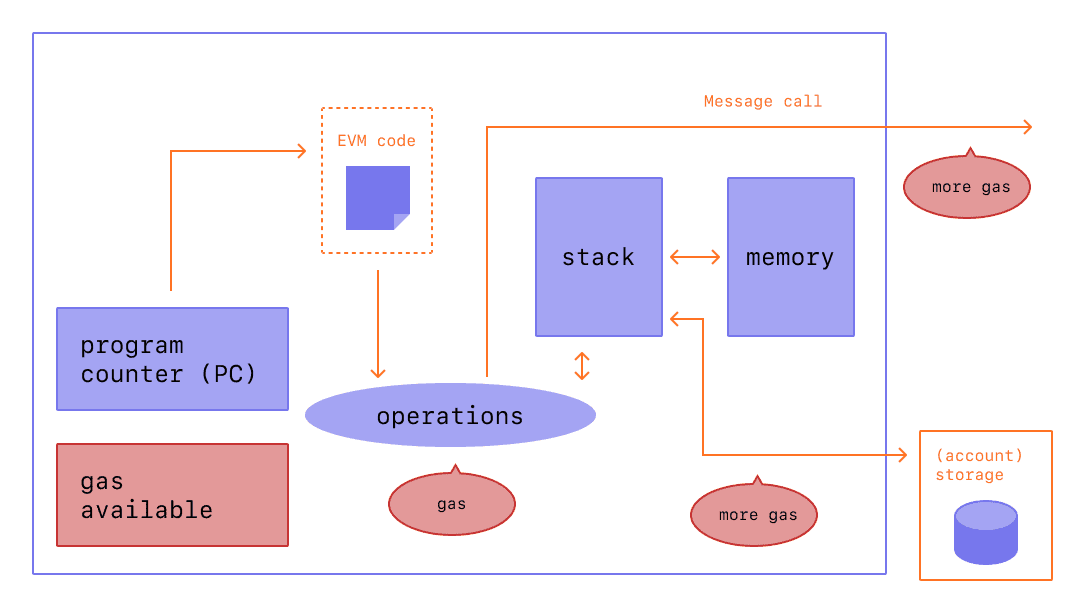
\includegraphics[width=400px]{images/gas.png}
\end{figure}

\textit{Gas} được trả bằng đồng \textit{ether} (ETH). \textit{Giá gas}\footnote{Gas price} có đơn vị là \textit{gwei}, mỗi \textit{gwei} tương ứng với một phần một tỷ của một \textit{ether}: $1$ \textit{gwei} $=10^{-9}$ \textit{ether}. Vì vậy, thay vì nói chi phí giao dịch là $0,000000001$ \textit{ether}, ta có thể nói giao dịch đó tiêu tốn $1$ \textit{gwei}. Ngoài ra, $1$ \textit{gwei} chính là một tỷ \textit{wei}; \textit{wei} (được đặt tên theo \textit{Wei Dai} - nhà khoa học máy tính nổi tiếng đưa ra lý thuyết về thanh toán bằng tiền mã hoá) là đơn vị nhỏ nhất trên Ethereum.\\

